\documentclass[pdf,ps,8pt]{beamer}

\usepackage{lmodern}
\usepackage{amsmath}
\usepackage{color}
\usepackage{bbold}
\usepackage{cancel}
\usepackage{slashed}
\usepackage{graphicx}
\usepackage{verbatim}
\usepackage{textcomp}

\usetheme{Singapore}

\definecolor{palegray}{rgb}{0.82,0.822,0.82}
\newcommand{\preliminary}{
{ \rput{30}(7,-4.0){\fontsize{40}{40}\selectfont {\color{palegray}Preliminary Preliminary}} }
}

\newcommand{\textapprox}{\raisebox{0.5ex}{\texttildelow}}

\newcommand{\miniscule}{\fontsize{3pt}{4pt}\selectfont}

\def\MSbar{$\overline{\mathrm{MS}}$}
\def\gev{\,\mathrm{GeV}}
\def\mev{\,\mathrm{MeV}}
\def\fm{\,\mathrm{fm}}
\def\SU{\mathrm{SU}}
\def\su#1#2{\SU(#1)_\mathrm{#2}}
\def\rpisq{\langle r_\pi^2\rangle}
% final values
\def\rpisqsim{0.38(4)}  % pole fit for 330 MeV pion
\def\rpisqsu2sim{0.354(31)}  % su2 fit for 330 MeV pion
\def\rpisqsimlong{0.382(42)}
\def\rpisqphys{0.418(31)} % SU(2) chi extrap
\def\rpisqphyslong{0.418(31)}
\def\lsixr{-0.0093(10)} % SU(2)
\def\Lniner{0.0031(6)}  % SU(3)

\newcommand{\chpt}{\chi^{\rm PT}}
\newcommand{\tchpt}{$\chi^{\rm PT}$}
\newcommand{\tchptthree}{$\chi^{\rm PT}_3$}
\newcommand{\tchpttwo}{$\chi^{\rm PT}_2$}

\newcommand{\xiav}{\langle\,\xi\,\rangle}
\newcommand{\xisqav}{\langle\,\xi^2\,\rangle}


\newcommand{\mD}{\left(\begin{array}{cc} \DO & \Dd \\  \Ddb&\DOb \end{array} \right)}

\newcommand{\Ob}{\bar{\Omega}}

\newcommand{\DO}{D_\Omega}
\newcommand{\Dd}{D_\partial}
\newcommand{\DOi}{D_\Omega^{-1}}
\newcommand{\DOid}{D_\Omega^{-\dagger}}
\newcommand{\Pd} {\mathbb{P}_\partial}
\newcommand{\PO} {\mathbb{P}_\Omega}

\newcommand{\DOb}{D_{\bar{\Omega}}}
\newcommand{\Ddb}{D_{\bar{\partial}}}
\newcommand{\DObi}{D_{\bar{\Omega}}^{-1}}
\newcommand{\DObid}{D_{\bar{\Omega}}^{-\dagger}}
\newcommand{\Pdb}{\mathbb{P}_{\bar{\partial}}}
\newcommand{\POb} {\mathbb{P}_{\bar\Omega}}

\newcommand{\Phidb}{\mathbb{\phi}_{\bar{\partial}}}
\newcommand{\etadb}{\mathbb{\eta}_{\bar{\partial}}}

\newcommand{\hDO}{\hat D_\Omega}
\newcommand{\hDd}{\hat D_\partial}
\newcommand{\hDOi}{\hat D_\Omega^{-1}}
\newcommand{\hPd} {\hat{\mathbb{P}}_\partial}

\newcommand{\hDOb}{\hat D_{\bar{\Omega}}}
\newcommand{\hDdb}{\hat D_{\bar{\partial}}}
\newcommand{\hDObi}{\hat D_{\bar{\Omega}}^{-1}}
\newcommand{\hPdb}{\hat{\mathbb{P}}_{\bar{\partial}}}

\newcommand{\mul}[1]{\left(\begin{array}{cc}#1 & 0 \\ 0& 0\end{array}\right)}
\newcommand{\mur}[1]{\left(\begin{array}{cc}0  & #1\\ 0& 0\end{array}\right)}
\newcommand{\mll}[1]{\left(\begin{array}{cc}0  & 0 \\ #1 & 0\end{array}\right)}
\newcommand{\mlr}[1]{\left(\begin{array}{cc}0  & 0 \\ 0& #1\end{array}\right)}

\newcommand{\mDO}{\mul{ \DO}}
\newcommand{\mDd}{\mur{ \Dd}}
\newcommand{\mDOi}{\mul{\DOi}}
\newcommand{\mPd} {\mlr{\Pd}}

\newcommand{\mDOb}{\mlr{\DOb}}
\newcommand{\mDdb}{\mll{\Ddb}}
\newcommand{\mDObi}{\mlr{\DObi}}
\newcommand{\mPdb}{\mul{\Pdb}}
\newcommand{\rmod}{\mathrm{mod}}
\newcommand{\rdiv}{\mathrm{div}}

\newcommand{\link}[1]{\href{#1}{ {\color{blue} #1} }}

\beamertemplatenavigationsymbolsempty
\begin{document}


\begin{frame}[fragile]\small\frametitle{  Computational Methods (practice) -  Lecture 4    }

  \begin{center}
 
  {\color{red} Peter Boyle} (BNL, Edinburgh)

  \begin{itemize}
  \item Monte Carlo Integration
  \item Euclidean path integral and HMC
  \item Pseudofermions
  \item Writing and running an HMC
  \item Odd flavours
  \end{itemize}

\end{center}  
\end{frame}

\begin{frame}[fragile]\small\frametitle{Monte Carlo Integration}
\begin{itemize}
\item Integration
  $$
  \int_U f(U) dU =  Vol \times \langle f \rangle  \quad \quad ; \quad \quad Vol = \int_U dU
  $$
\item Monte Carlo Integration ($x_i$ uniform over compact domain)
  $$
  \langle f \rangle = \frac{1}{N}\sum\limits_i f(x_i)
  $$
\item Importance sampling: draw $x_i$ with positive normalised probability density $P(x_i)$
  $$
  \langle f \rangle = \frac{1}{N}\sum\limits_i \frac{f(x_i)}{P(x_i)}
  $$
\item If $|f(x_i)| \propto P(x_i)$ this may converge better.

\item Variance reduction: if $\tilde{f}$ is a good, cheap approximation for $f$
  $$
  \langle f \rangle = \frac{1}{N\times M}\sum\limits_i \frac{\tilde{f}(x_i)}{P(x_i)}
                    + \frac{1}{N}\sum\limits_j \frac{f(x_j) - \tilde{f}(x_j)}{P(x_j)}
  $$
\end{itemize}
\end{frame}

\begin{frame}[fragile]\small\frametitle{Euclidean Path Integral}
\begin{itemize}
\item Pure gauge path integral
  $$
  \frac{1}{Z} \int_U e^{-S_G[U]} {\cal O}(U) dU 
  $$
\item Importance sample: seek to distribute gluon configuratoins according to
  $$
  P(U) = \frac{e^{-S_G[U]}}{\int_U e^{-S_G[U]} dU}
  $$
\item Calculate observables on each \emph{configuration}
  $$
\langle {\cal O} \rangle = \frac{1}{N} \sum\limits_i {\cal O}(U_i) 
$$
\item $\Rightarrow$ Markov chain monte carlo:
\begin{itemize}
\item $10^{10}$ degrees of freedom(!)
\item Sharply probability weight
\item Variance of ${\cal O}(U)$ determines how many samples are required.
\item 100-2000 samples typically good for 1\% scale statistical errors
\end{itemize}
\item This is observable dependent...  
\end{itemize}
\end{frame}


\begin{frame}[fragile]\small\frametitle{Markov chains}
  \begin{itemize}
\item Sequence of states generated by \emph{transition probability} $M(X\to X^\prime)$ from $X$ to $X^\prime$\\
      Rule depends only on $X$.
\item Usually composed of proposal and acceptance probablities
$$
M(X\to X^\prime) = P_p(X\to X^\prime) P_{acc}(X\to X^\prime)
$$
\item Design rule $M(X\to X^\prime)$ to yield \emph{desired} equilibrium probability distribution after many transitions$P_{eq}(X)$
\item $P_{eq}$ must map to itself under of the transition rule:
$$
P_{eq}(X^\prime) = \sum\limits_X P_{eq}(X) M(X \to X^\prime) 
$$
\item An ergodic update satisfying this \emph{and} is a contration mapping leads to
      Markov transitions converge on the desired equilibrium.
  \end{itemize}
(Clear pedagogical review: Anthony Kennedy Nara lectures 2006)
\end{frame}

\begin{frame}[fragile]\small\frametitle{Metropolis algorithms}
  \begin{itemize}
  \item Detailed balance property:
$$
P_{eq}(X) M(X\to X^\prime) = P_{eq}(X^\prime) M(X^\prime\to X)
$$
\item Sum over $X$ to obtain
$$
\sum\limits_X P_{eq}(X) M(X\to X^\prime) = \sum\limits_X P_{eq}(X^\prime) M(X^\prime\to X)= P_{eq}(X^\prime) 
$$
\item So $P_{eq}$ is a \emph{fixed point} of the Markov process!
\item \fbox{We can sample any probability distribution we desire with such an update.}
\end{itemize}
\end{frame}

\begin{frame}[fragile]\small\frametitle{Metropolis algorithms}
\begin{itemize}
\item Make the update combine proposal and acceptance probablities
$$
M(X\to X^\prime) = P_p(X\to X^\prime) P_{acc}(X\to X^\prime)
$$
\item detailed balance
$$
P_{eq}(X) P_p(X\to X^\prime) P_{acc}(X\to X^\prime) = P_{eq}(X^\prime)  P_p(X^\prime\to X) P_{acc}(X^\prime\to X ),
$$
\item is satisfied with the Metropolis acceptance probability, 
$$
P_{acc}(X\to X^\prime) = {\rm Min} ( 1, \frac{P_{eq}(X^\prime)  P_p(X^\prime\to X)}{P_{eq}(X) P_p(X\to X^\prime) } )
$$
\item either $P_{acc}(X\to X^\prime) = 1$, or $P_{acc}(X^\prime\to X)$; considering cases leads to trivial proof.
\item Simplifies if $P_p(X^\prime\to X) = P_p(X\to X^\prime)$ (reversible, area preserving constraint)
\end{itemize}
\begin{center}
  \fbox{Basis of most Markov Chain Monte Carlo}
\end{center}
\end{frame}

\begin{frame}[fragile]\small\frametitle{QCD path integral}

\begin{itemize}
\item Partition function becomes a real, statistical mechanical probability weight
  $$Z= \int d\bar\psi d\psi d U e^{-S_G[U]- S_F[\bar\psi,\psi,U]}$$
\item Dirac differential operator represented via discrete derivative approximations: sparse matrix
\item Use pseudofermion approach to replace with Gaussian integral $\sqrt{\pi\lambda} = \int dt e^{-t^2/\lambda}$
$$
\int {\cal D}\bar \psi {\cal D\psi} e^{-\bar\psi(x) A_{xy} \psi(y) } = \det A
$$
$$
\pi \lambda = \int d\phi_r e^{-\phi_r \frac{1}{\lambda}  \phi_r}
              \int d\phi_i e^{-\phi_i \frac{1}{\lambda}  \phi_i} 
              = \int d\phi^\ast d\phi e^{-\phi^\ast \frac{1}{\lambda}  \phi}
$$
\item replace two flavour determinant with a two flavour \emph{pseudofermion} integral
$$
(\det M)^2 = (\det \gamma_5 M)^2 = \det M^\dag M = \int {\cal D}\phi^\ast {\cal D} \phi e^{-\phi^\ast(x) (M^\dag M)^{-1} \phi(y) }
$$
\end{itemize}

\end{frame}

\begin{frame}[fragile]\small\frametitle{Hybrid Monte Carlo}
\begin{itemize}
\item Auxiliary Gaussian integral over conjugate momentum field $\int d\pi e^\frac{-\pi^2}{2}$ \\
  Lives in Lie algbra; serves only to move $U$ round the group Manifold
  $$
  \int d\pi
  \int d \phi
  \int d U \quad
  e^{-\frac{\pi^2}{2}}
  e^{-S_G[U]}
  e^{-\phi^\ast (M^\dag M)^{-1} \phi }
  $$
\item Outer Metropolis Monte Carlo algorithm
  \begin{itemize}
  \item Draw momenta
  \item Draw pseudofermion as gaussian $\eta = M^{-1} \phi$
  \item Metropolis acceptance step
  \end{itemize}
\item Metropolis proposal includes {inner molecular dynamics} at constant Hamiltonian:
  $$
  H= \frac{\pi^2}{2}+S_G[U]+\phi^\ast (M^\dag M)^{-1} \phi
  $$
  $$\dot{U} = i \pi U \quad\quad;\quad\quad i \dot \pi = - ( U \nabla_U S)_{TA}$$
\item {\color{red} Must invert $M^\dagger M$ at each timestep of evolution in MD force }
$$\delta (M^\dag M)^{-1} = -  (M^\dag M)^{-1} [(\delta M^\dag) M + M (\delta M) ] (M^\dag M)^{-1}$$
\end{itemize}
\end{frame}

\begin{frame}[fragile]\small\frametitle{Force terms \& conventions }

  Derive from:
  $$
  \dot{H} = 0 = \pi \left[ \dot \pi + i  U \cdot \nabla_U S_{TA} \right]
  $$
  \begin{itemize}
   \item Define \emph{force} as the rate of change of momentum and is calculated by differentiating
     action with respect to each element of each link (and multiplying by $U_\mu$ ; leaving untraced).
   \item Grid ``derivative'' functions have some notable conventions. These simplify code but make somewhat non-obvious
   \item All code bases I have read have such quirks(!)
  \begin{enumerate}
     \item $p_\mu = i p^a \tau^a $, removes factor of $i$ in exponentiation
     \item Real actions (which we need for importance sampling) depend on $U$ and $U^\dagger$ in a symmetric way.
     \item ``really'' should calculate $dS/dU$ and $dS/dU^\dagger$ but this is a factor of two.
     \item ``actually'' calculate $dS/dU$ and take the traceless anti-hermitian part: leaves an implicit factor of two in force included in integrator.
  \end{enumerate}
  \item Finite timestep of U is performed in the Lie algebra: $U^\prime = e^{i \pi dt} U$, keeping U on the group manifold
  \item Force terms reduce to simple application of the product and chain rule, bearing in mind the rules of matrix differentiation.
  \item Code is typically pretty well commented and self documenting
  \end{itemize}

\end{frame}

  
\begin{frame}[fragile]\small\frametitle{ Pseudofermion options }

\link{https://github.com/paboyle/Grid/tree/develop/Grid/qcd/action/pseudofermion}

\begin{columns}
\begin{column}{0.75\textwidth}
\begin{itemize}
\item Recall ${\rm det} M = {\rm det} M_{pc} {\rm det} M_{ee}$
\item Require symmetric positive definite Gaussian integral (\emph{not} just positive ${\rm det} M$ )
\item Two degenerate flavours is easy: $\phi^\dagger M^\dagger M \phi$
\item Odd flavours harder: take square root of $\phi^\dagger M^\dagger M \phi$ in HPD fashion
\item Polynomial HMC (Chebyshev) and Rational HMC (c.f. num rep)
\item \emph{Require positivity of one flavour determinant} 
\begin{itemize}
\item Guaranteed for DWF with positive mass, but not for Wilson (expected for sufficiently large mass, exceptional configurations are light mass)
\item \link{https://arxiv.org/abs/2003.13359}: \emph{In the simulation of QCD with 2+1 flavors of Wilson fermions, the positivity of the fermion determinant is generally assumed. We present evidence that this assumption is in general not justified and discuss the consequences of this finding.}
\item For DWF exact one flavour algorithm also
\end{itemize}
\item RHMC efficient due to \emph{multi-shift solvers}
\end{itemize}
\end{column}
\begin{column}{0.25\textwidth}
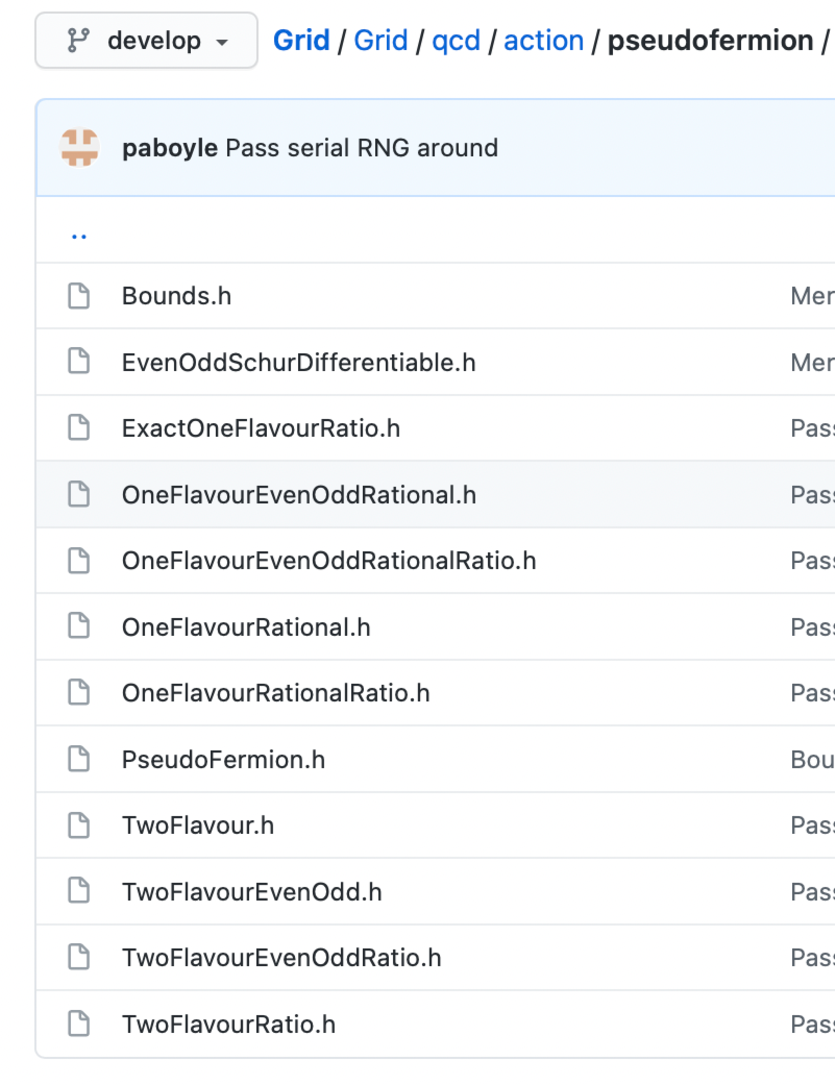
\includegraphics[width=\textwidth]{Pseudofermion.pdf}
\end{column}
\end{columns}
\end{frame}

\begin{frame}[fragile]\small\frametitle{ Integrators }
\begin{itemize}
\item Integrators should be area preserving to keep phase space density same $\Rightarrow$ symplectic integrators
\item Integrators can be nested (Sexton-Weingarten) to integrate different action fragments on different timescales
\begin{itemize}
\item e.g. Gauge force is nearly free to evaluate
\end{itemize}
\item Integrators can be nested (Sexton-Weingarten) to integrate different action fragments on different timescales
\item Leapfrog, Omelyan, Force Gradient give different orders of integration error in $\delta t$ 
\item Peak determinant force can be reduced using a series of \emph{Hasenbusch determinant ratios}
\item Tuning determinant factoring and timesteps is laborious and empirical
\item Practical recommendation: 
\begin{itemize}
\item Factor determinants and place all on same timescale, use Force Gradient
\item Balance forces between pseudofermion factors
\item Increase fermion timestep until acceptance drops to 90\%
\item Integrate gauge action on a sufficiently fine resolution that delta Hamiltonian is independent of gauge timestep
\end{itemize}
\end{itemize}
\end{frame}

\begin{frame}[fragile]\small\frametitle{ Pseudofermion code example }

  \link{https://github.com/paboyle/Grid/blob/develop/Grid/qcd/action/pseudofermion/TwoFlavourRatio.h}
  {  \tiny
\begin{verbatim}
      FermionOperator<Impl> & NumOp;// the basic operator
      FermionOperator<Impl> & DenOp;// the basic operator

      OperatorFunction<FermionField> &DerivativeSolver;
      OperatorFunction<FermionField> &ActionSolver;
      OperatorFunction<FermionField> &HeatbathSolver;

      FermionField PhiOdd;   // the pseudo fermion field for this trajectory
      FermionField PhiEven;  // the pseudo fermion field for this trajectory
  \end{verbatim}
    }
\end{frame}


\begin{frame}[fragile]\small\frametitle{ Pseudofermion code example }
\link{https://github.com/paboyle/Grid/blob/develop/Grid/qcd/action/pseudofermion/TwoFlavourRatio.h}
  {  \tiny
\begin{verbatim}
  //////////////////////////////////////////////////////
  // S = phi^dag V (Mdag M)^-1 Vdag phi
  //////////////////////////////////////////////////////
  virtual RealD S(const GaugeField &U) {

    NumOp.ImportGauge(U);
    DenOp.ImportGauge(U);

    FermionField X(NumOp.FermionGrid());
    FermionField Y(NumOp.FermionGrid());
	
    MdagMLinearOperator<FermionOperator<Impl> ,FermionField> MdagMOp(DenOp);

    NumOp.Mdag(Phi,Y);              // Y= Vdag phi
    X=Zero();
    ActionSolver(MdagMOp,Y,X);      // X= (MdagM)^-1 Vdag phi
    DenOp.M(X,Y);                  // Y=  Mdag^-1 Vdag phi

    RealD action = norm2(Y);

    return action;
  };
\end{verbatim}
}
\end{frame}


\begin{frame}[fragile]\small\frametitle{ Pseudofermion code example }
\link{https://github.com/paboyle/Grid/blob/develop/Grid/qcd/action/pseudofermion/TwoFlavourRatio.h}
  {  \tiny
\begin{verbatim}
  //////////////////////////////////////////////////////
  // dS/du = phi^dag dV (Mdag M)^-1 V^dag  phi
  //       - phi^dag V (Mdag M)^-1 [ Mdag dM + dMdag M ]  (Mdag M)^-1 V^dag  phi
  //       + phi^dag V (Mdag M)^-1 dV^dag  phi
  //////////////////////////////////////////////////////
  virtual void deriv(const GaugeField &U,GaugeField & dSdU) {

    NumOp.ImportGauge(U);
    DenOp.ImportGauge(U);

    MdagMLinearOperator<FermionOperator<Impl> ,FermionField> MdagMOp(DenOp);

    FermionField  X(NumOp.FermionGrid());
    FermionField  Y(NumOp.FermionGrid());
    GaugeField   force(NumOp.GaugeGrid());	

    //Y=Vdag phi
    //X = (Mdag M)^-1 V^dag phi
    //Y = (Mdag)^-1 V^dag  phi
    NumOp.Mdag(Phi,Y);              // Y= Vdag phi
    X=Zero();
    DerivativeSolver(MdagMOp,Y,X);      // X= (MdagM)^-1 Vdag phi
    DenOp.M(X,Y);                  // Y=  Mdag^-1 Vdag phi

    // phi^dag V (Mdag M)^-1 dV^dag  phi
    NumOp.MDeriv(force , X, Phi, DaggerYes );  dSdU=force;
  
    // phi^dag dV (Mdag M)^-1 V^dag  phi
    NumOp.MDeriv(force , Phi, X ,DaggerNo  );  dSdU=dSdU+force;

    //    -    phi^dag V (Mdag M)^-1 Mdag dM   (Mdag M)^-1 V^dag  phi
    //    -    phi^dag V (Mdag M)^-1 dMdag M   (Mdag M)^-1 V^dag  phi
    DenOp.MDeriv(force,Y,X,DaggerNo);   dSdU=dSdU-force;
    DenOp.MDeriv(force,X,Y,DaggerYes);  dSdU=dSdU-force;

    dSdU *= -1.0;
  };
\end{verbatim}
}
\end{frame}

\begin{frame}[fragile]\small\frametitle{ Pseudofermion code example }

\link{https://github.com/paboyle/Grid/blob/develop/Grid/qcd/action/pseudofermion/TwoFlavourRatio.h}
  {  \tiny
\begin{verbatim}
  virtual void refresh(const GaugeField &U, GridSerialRNG &sRNG, GridParallelRNG& pRNG) {

    // P(phi) = e^{- phi^dag V (MdagM)^-1 Vdag phi}
    //
    // NumOp == V
    // DenOp == M
    //
    // Take phi = Vdag^{-1} Mdag eta  ; eta = Mdag^{-1} Vdag Phi
    //
    // P(eta) = e^{- eta^dag eta}
    //
    // e^{x^2/2 sig^2} => sig^2 = 0.5.
    // 
    // So eta should be of width sig = 1/sqrt(2) and must multiply by 0.707....
    //
    RealD scale = std::sqrt(0.5);

    FermionField eta(NumOp.FermionGrid());
    FermionField tmp(NumOp.FermionGrid());

    gaussian(pRNG,eta);

    NumOp.ImportGauge(U);
    DenOp.ImportGauge(U);

    // Note: this hard codes normal equations type solvers; alternate implementation needed for 
    // non-herm style solvers.
    MdagMLinearOperator<FermionOperator<Impl> ,FermionField> MdagMOp(NumOp);

    DenOp.Mdag(eta,Phi);            // Mdag eta
    tmp = Zero();
    ActionSolver(MdagMOp,Phi,tmp);  // (VdagV)^-1 Mdag eta = V^-1 Vdag^-1 Mdag eta
    NumOp.M(tmp,Phi);               // Vdag^-1 Mdag eta

    Phi=Phi*scale;
	
  };
\end{verbatim}
}
\end{frame}

\begin{frame}[fragile]\small\frametitle{Even Odd preconditioning}
\begin{itemize}
\item We can write the Fermion determinant in terms of the red-black preconditioned operator
$$
M = \left(
\begin{array}{cc}
M_{ee} & M_{eo} \\
M_{oe} & M_{oo}
\end{array}
\right)
= 
\left(
\begin{array}{cc}
1  &  0 \\
M_{oe} M_{ee}^{-1}  & 1
\end{array}
\right)
\left(
\begin{array}{cc}
M_{ee} & 0\\
0 & M_{oo} - M_{oe}M_{ee}^{-1} M_{eo}
\end{array}
\right)
\left(
\begin{array}{cc}
1 &  M_{ee}^{-1}M_{eo}\\
0  & 1
\end{array}
\right),
$$
\item where the Schur complement, is written as $M_{pc} = M_{oo} - M_{oe}M_{ee}^{-1} M_{eo}$.
\item $\det U = \det M = 1$ and so,
$$
\det M = \det M_pc \det M_{ee}
$$
\item Since the inverse of $M_{pc}^\dagger M_{pc}$ arises from a conjugate gradient solve (making the matrix HPD), 
and $M_{pc}^{-dagger} = M_{pc} (M_{pc}^\dagger M)^{-1}$, we can use both red-black solvers and a single solve 
in the force evaluation by using the Schur factored determinant in HMC.
\end{itemize}
\end{frame}

\begin{frame}[fragile]\small\frametitle{Observables}

Importance sampling has reduced:
$$
\langle {\cal O} \rangle = \frac{1}{Z} \int_U e^{-S_G[U]} {\cal O}(U) dU  \to \frac{1}{N} \sum\limits_i {\cal O}(U_i) 
$$
\begin{itemize}
\item Zero momentum pion, kaon or B meson two point function
  $$
  \sum\limits_x \langle \bar u \gamma_0 \gamma_5 d (x,t) \bar d \gamma_0 \gamma_5 u (0,0) \rangle
    = \frac{1}{N}\sum_i  {\rm trace}  \{ \gamma_0 \gamma_5 M^{-1}_d(x,t;0,0)\gamma_0 \gamma_5 M^{-1}_u(0,0;x,t) \}
    $$
\item Euclidean space $\propto A e^{- m t} $
\item Tune bare mass until interacting meson mass is correct, prefactor gives pion, kaon, B meson decay constant
\item etc.. 
\end{itemize}
  
\end{frame}


\begin{frame}[fragile]\small\frametitle{Exercise}

\begin{itemize} 
\item Quenched simulation for Gauge action of your choice
\item Create a corresponding Grid HMC: cut down the Mobius DWF HMC as required
\item Run it on your laptop on $8^4$ and check you get close to the same plaquette as literature results
  \begin{itemize}
    \item e.g. https://arxiv.org/pdf/hep-lat/0610075.pdf
    \end{itemize}
\item Check the Creutz relation: $<e^{-dH}> = 1$
\item Save the gauge configurations for the next lecture(!)
\end{itemize}

Examples:

\link{https://github.com/paboyle/Grid/blob/develop/HMC/Mobius2p1fRHMC.cc}

\link{https://github.com/paboyle/Grid/tree/develop/tests/hmc}

\end{frame}


\begin{frame}[fragile]\small\frametitle{Resources}

\begin{itemize}
\item \href{https://inspirehep.net/literature/254077}{\color{blue}Kennedy, Pendleton, Roweth, Duane HMC}
\item \href{https://inspirehep.net/literature/31867}{\color{blue}Sexton-Weingarten}
\item \href{https://inspirehep.net/literature/560630}{\color{blue}Hasenbusch determinant factoring}
\item \href{https://inspirehep.net/literature/628174}{\color{blue}Kennedy, Clark RHMC}
\end{itemize}

Topics not covered:

\begin{itemize}
  \item Link smearing
  \item Exact one flavor algorithm (DWF)
  \item DDHMC
  \item Multigrid setup in HMC and polynomial subspace prediction
  \item Multishift solvers
  \item Polynomial HMC
\end{itemize}

\end{frame}

\end{document}



